\documentclass[a4paper,12pt]{article}

\usepackage[utf8]{inputenc}
\usepackage[T1]{polski}
\usepackage{helvet}
\usepackage{graphicx}
\usepackage{color}
\usepackage{xcolor}
\usepackage{geometry}
\usepackage{caption}
\usepackage{makeidx}
\usepackage{multirow}
\usepackage{wrapfig}
\usepackage{listings}


\geometry{hmargin={2cm, 2cm}, height=10.0in}
\DeclareCaptionFont{white}{\color{white}}
\DeclareCaptionFormat{listing}{\colorbox{gray}{\parbox{\textwidth}{#1#2#3}}}
\captionsetup[lstlisting]{format=listing,labelfont=white,textfont=white}
\lstset{ %
language=Octave,                % choose the language of the code
basicstyle=\footnotesize,       % the size of the fonts that are used for the code
numbers=left,                   % where to put the line-numbers
numberstyle=\footnotesize,      % the size of the fonts that are used for the line-numbers
stepnumber=1,                   % the step between two line-numbers. If it's 1 each line 
                                % will be numbered
numbersep=5pt,                  % how far the line-numbers are from the code
backgroundcolor=\color{white},  % choose the background color. You must add \usepackage{color}
showspaces=false,               % show spaces adding particular underscores
showstringspaces=false,         % underline spaces within strings
showtabs=false,                 % show tabs within strings adding particular underscores
frame=single,	                % adds a frame around the code
tabsize=2,	                % sets default tabsize to 2 spaces
%captionpos=b,                   % sets the caption-position to bottom
breaklines=true,                % sets automatic line breaking
breakatwhitespace=false,        % sets if automatic breaks should only happen at whitespace
title=\lstname,                 % show the filename of files included with \lstinputlisting;
                                % also try caption instead of title
escapeinside={\%*}{*)},         % if you want to add a comment within your code
morekeywords={*,...}            % if you want to add more keywords to the set
}

\lstloadlanguages{ Ruby }


\makeindex

\begin{document}

% =====  STRONA TYTULOWA PRACY INŻYNIERSKIEJ ====
% ostatnia modyfikacja: 2009/07/01, K. Malarz

\thispagestyle{empty}

%% ------------------------ NAGLOWEK STRONY ---------------------------------
\begin{figure}
\vspace{-13cm}
\hspace{-4cm}

\includegraphics[height=29.3cm]{grafika/agh_nzw_a_pl_1w_wbr_cmyk.pdf}\\
\vspace{-13.9cm}
\end{figure}
\rule{26mm}{0pt}
{\large\textsf{Wydział Fizyki i Informatyki Stosowanej}}\\
\rule{\textwidth}{3pt}\\
\rule[2ex]
{\textwidth}{1pt}\\
\vspace{7ex}
\begin{center}
{\bf\LARGE\textsf{Analiza i przetwarzanie obrazów}}\\
\vspace{13ex}
{\bf\huge\textsf{Ćwiczenie 2}}\\
\vspace{3ex}
{\sf \small } {\bf\small\textsf{Krystian Wojtas}}\\
\vspace{14ex}
%% ------------------------ OPIEKUN PRACY ------------------------------------
{\sf \Large } {\bf\Large\textsf{}}\\
\vspace{22ex}
\textsf{\bf\large\textsf{Kraków, październik 2011}}
\end{center}
%% =====  STRONA TYTUŁOWA PRACY INŻYNIERSKIEJ  ====


\newpage
\section{Wstęp}
Celem ćwiczeń było skalowanie, progowanie oraz filtrowanie obrazu. Wykorzystany został język Ruby i jego framework RMagic, który binduje funkcje biblioteczne z pakietu ImageMagick.

\subsection{Obraz przetwarzany}
\begin{figure}[h!]
   \centering
   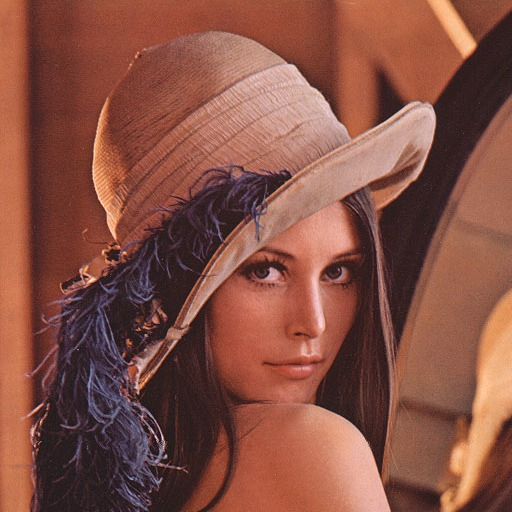
\includegraphics[width=15cm]{../../lena.jpg}
   \caption{Obraz poddawany obróbce}
\end{figure}


\newpage
\section{Skalowanie}
Obraz ulega zmianie rozmiarów poprzez przepisanie wartości kolorów pikseli w nowych położeniach. Pomniejszając, przepisane zostaną tylko wybrane okresowo piksele. Powiększjąc, ten sam piksel orginału zostanie zapisany w kilku położeniach wypełniająć w ten sposób dodatkowy obszar.

Do skalowania użyty został wzór
$$p(x, y) = p(x/skala, y/skala)$$
\begin{figure}[h!]
   \centering
   \includegraphics[width=15cm]{../out/zoom40.jpg}
   \caption{Skala 4.0}
\end{figure}
\begin{figure}[h!]
   \centering
   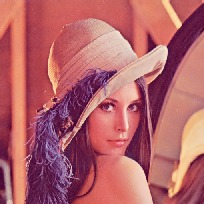
\includegraphics[width=15cm]{../out/zoom04.jpg}
   \caption{Skala 0.4}
\end{figure}

\newpage
Oba obrazy mają w sprawozdaniu po 15cm szerokości jak obraz wzorcowy. Są one wyskalowywane przez program latex do tych rozmiwarów. Dlatego między wzorcem a obrazem powiększonym 1.5x, a następnie ponownym wyskalowaniu do 15cm szerokości nie widać istotnych różnic.


W przypadku pomniejszenia w skali 0.4x, obraz skurczył się do rozmiarów 204x204 i utracił sporo informacji. Po ponownym wyskalowaniu do 15cm szerokości strony, zauważyć można znaczną utratę jakości, obraz stał się poszarpany, uwidaczniają się poszczególne piksele.

\lstinputlisting[caption=Implementacja efektu skalowania]{listingi/zoom.rb}


\section{Filtry}

\begin{figure}[h!]
\begin{minipage}[t]{7.5cm}
\begin{center}
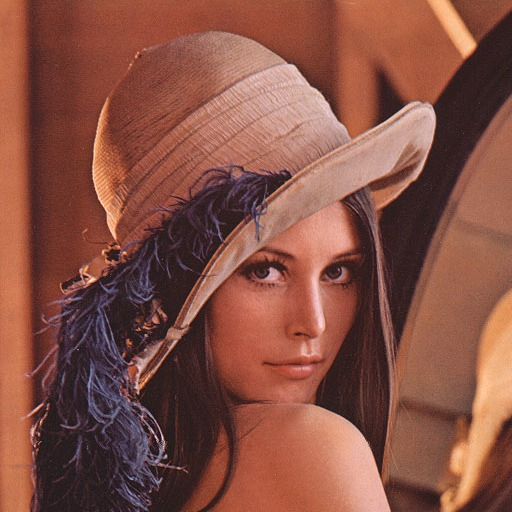
\includegraphics[width=7.5cm,clip]{../../lena.jpg}
\caption{Wzorzec}
\end{center}
\end{minipage}
\hfill
\begin{minipage}[t]{7.5cm}
\begin{center}
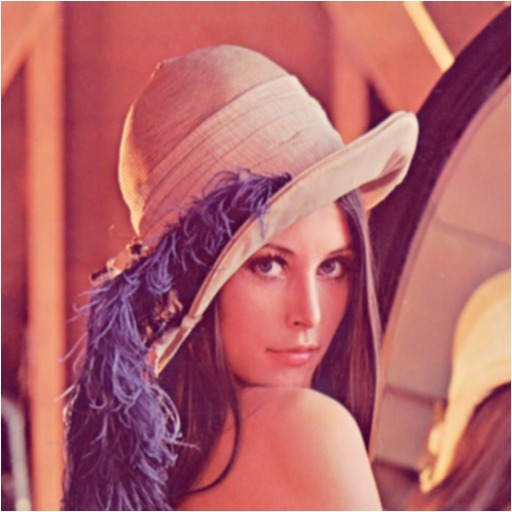
\includegraphics[width=7.5cm,clip]{../out/fusr1.jpg}
\caption{Filtr uśredniający 1}
\end{center}
\end{minipage}
\end{figure}

\begin{figure}[h!]
\begin{minipage}[t]{7.5cm}
\end{minipage}
\hfill
\begin{minipage}[t]{7.5cm}
\begin{center}
\[ \left( \begin{array}{ccc}
1 & 1 & 1 \\
1 & 1 & 1 \\
1 & 1 & 1 \end{array} \right)\] 
\end{center}
\end{minipage}
\end{figure}

\begin{figure}[h!]
\begin{minipage}[t]{7.5cm}
\begin{center}
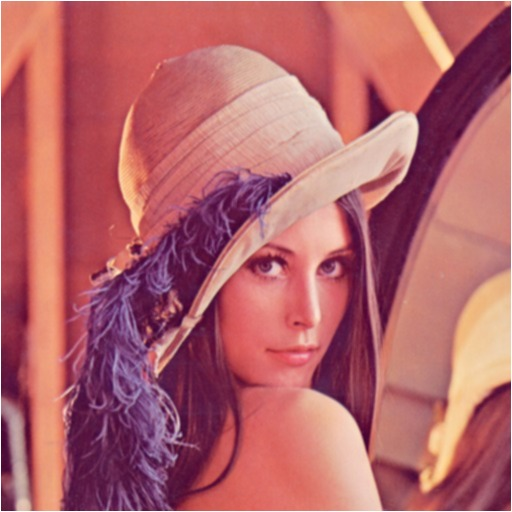
\includegraphics[width=7.5cm,clip]{../out/fusr2.jpg}
\caption{Filtr uśredniający 2}
\end{center}
\end{minipage}
\hfill
\begin{minipage}[t]{7.5cm}
\begin{center}
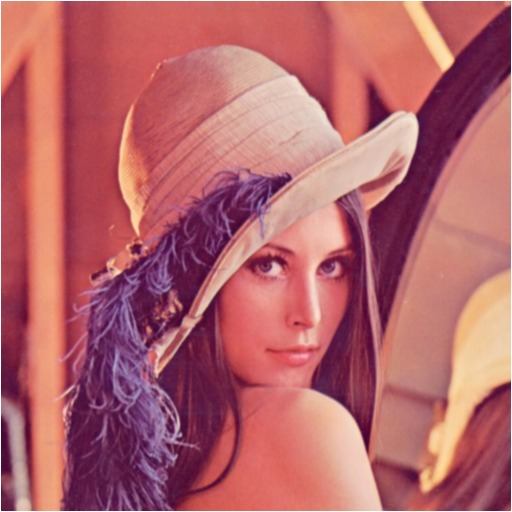
\includegraphics[width=7.5cm,clip]{../out/fusr3.jpg}
\caption{Filtr uśredniający 3}
\end{center}
\end{minipage}
\end{figure}

\begin{figure}[h!]
\begin{minipage}[t]{7.5cm}
\begin{center}
\[ \left( \begin{array}{ccc}
1 & 1 & 1 \\
1 & 2 & 1 \\
1 & 1 & 1 \end{array} \right)\] 
\end{center}
\end{minipage}
\hfill
\begin{minipage}[t]{7.5cm}
\begin{center}
\[ \left( \begin{array}{ccc}
1 & 2 & 1 \\
2 & 4 & 2 \\
1 & 2 & 1 \end{array} \right)\] 
\end{center}
\end{minipage}
\end{figure}




\newpage
\begin{figure}[h!]
\begin{minipage}[t]{7.5cm}
\begin{center}
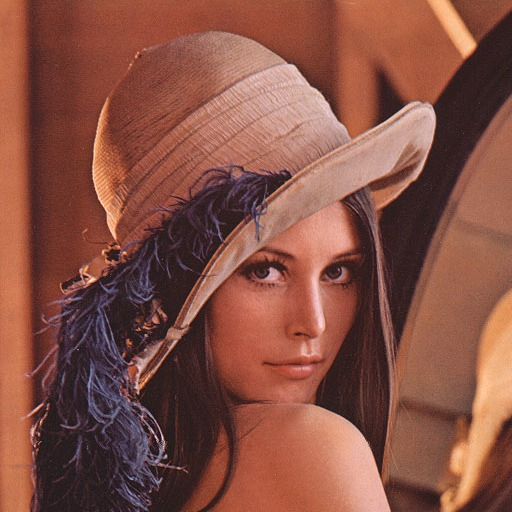
\includegraphics[width=7.5cm,clip]{../../lena.jpg}
\caption{Wzorzec}
\end{center}
\end{minipage}
\hfill
\begin{minipage}[t]{7.5cm}
\begin{center}
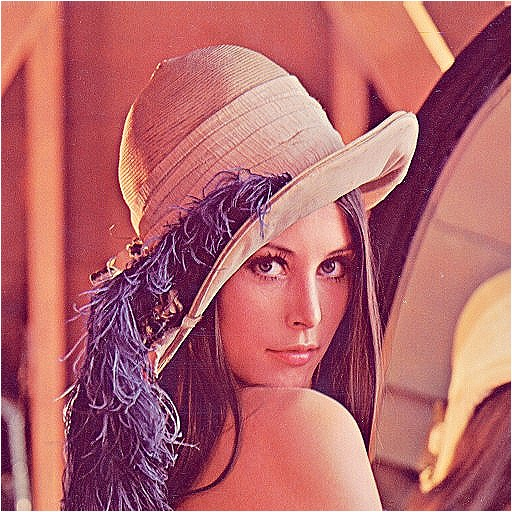
\includegraphics[width=7.5cm,clip]{../out/fwyostrz1.jpg}
\caption{Filtr wyostrzający 1}
\end{center}
\end{minipage}
\end{figure}

\begin{figure}[h!]
\begin{minipage}[t]{7.5cm}
\end{minipage}
\hfill
\begin{minipage}[t]{7.5cm}
\begin{center}
\[ \left( \begin{array}{ccc}
0 & -1 & 0 \\
-1 & 5 & -1 \\
0 & -1 & 0 \end{array} \right)\] 
\end{center}
\end{minipage}
\end{figure}

\begin{figure}[h!]
\begin{minipage}[t]{7.5cm}
\begin{center}
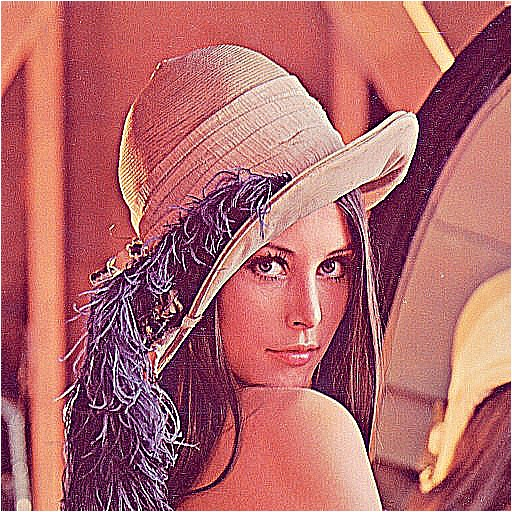
\includegraphics[width=7.5cm,clip]{../out/fwyostrz2.jpg}
\caption{Filtr wyostrzający 2}
\end{center}
\end{minipage}
\hfill
\begin{minipage}[t]{7.5cm}
\begin{center}
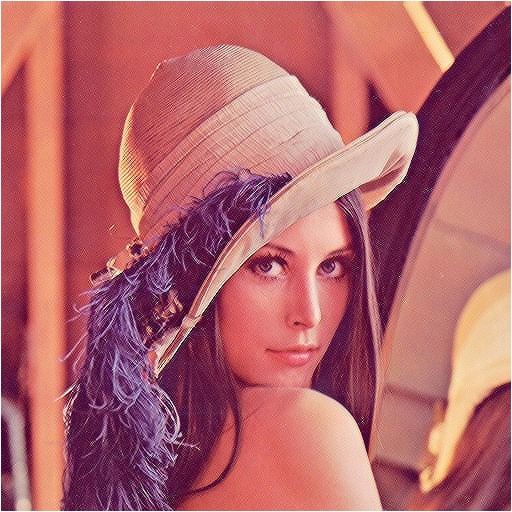
\includegraphics[width=7.5cm,clip]{../out/fwyostrz3.jpg}
\caption{Filtr wyostrzający 3}
\end{center}
\end{minipage}
\end{figure}

\begin{figure}[h!]
\begin{minipage}[t]{7.5cm}
\begin{center}
\[ \left( \begin{array}{ccc}
-1 & -1 & -1 \\
-1 & 9 & -1 \\
-1 & -1 & -1 \end{array} \right)\] 
\end{center}
\end{minipage}
\hfill
\begin{minipage}[t]{7.5cm}
\begin{center}
\[ \left( \begin{array}{ccc}
1 & -2 & 1 \\
-2 & 5 & -2 \\
1 & -2 & 1 \end{array} \right)\] 
\end{center}
\end{minipage}
\end{figure}


\newpage
W stosowanych filtrach wartość składowych poszczególnych barw uśrednia się wartościami sąsiadów przy zastosowaniu określonych ich wag - maski filtra.
Filtr uśredniający powoduje rozmazanie obrazu, utratę ostrości. Różnicę między orginałem a pierwszym filtrem widać dopiero w powiekszeniu. Mocniejsze filtry uśredniające nie przynoszą dostrzegalnych rezultatów.
Filtry wyostrzające dają wyraźny efekt.


\lstinputlisting[caption=Implementacja filtrów]{listingi/filter.rb}


\newpage
\section{Progowanie}

Progowanie oznacza przekształcenie obrazu określonego skalą szarości do postaci czarno-białej na podstawie zadanej wartości progu. Próg wyznacza się poprzez wcześniejsze wyliczenie średniej wartośći pikseli na obrazie.

\begin{figure}[h!]
\begin{minipage}[t]{7.5cm}
\begin{center}
\includegraphics[width=7.5cm,clip]{../out/prog.jpg}
\caption{Progowanie, prog = Magick::QuantumRange/2 = 32767}
\end{center}
\end{minipage}
\hfill
\begin{minipage}[t]{7.5cm}
\begin{center}
\includegraphics[width=7.5cm,clip]{../out/prog1.jpg}
\caption{Progowanie, prog jest srednia z wszystkich pikseli 32952}
\end{center}
\end{minipage}
\end{figure}

Średnia wartości wszystkich pikseli na obrazku wynosi 32952. Jest bardzo zbliżona do połowy zakresu Magick::QuantumRange/2 = 32767, stąd tak duże podobieństwo obu przekształceń. Jednakże różnice są dostrzegalne, przede wszystkim w zgrupowaniach naprzemiennych kropek białych i czarnych - miejsca, gdzie wartości pikseli są bardzo zbliżone do założonego progu np. w prawym górnym rogu. 

\lstinputlisting[caption=Progowanie]{listingi/thresholding.rb}

\subsection{Progowanie lokalne}

Obraz można podzielić na mniejsze fragmenty i w nich lokalnie obliczać średnią wartość oraz lokalnie progować względem tej wartości.

\newpage
\begin{figure}[h!]
\begin{minipage}[t]{6.5cm}
\begin{center}
\includegraphics[width=6.5cm,clip]{../out/prog1.jpg}
\caption{lokalnie 1 fragment}
\end{center}
\end{minipage}
\hfill
\begin{minipage}[t]{6.5cm}
\begin{center}
\includegraphics[width=6.5cm,clip]{../out/prog2.jpg}
\caption{lokalnie 4 fragmenty}
\end{center}
\end{minipage}
\end{figure}

\begin{figure}[h!]
\begin{minipage}[t]{6.5cm}
\begin{center}
\includegraphics[width=6.5cm,clip]{../out/prog4.jpg}
\caption{lokalnie 16 fragmentów}
\end{center}
\end{minipage}
\hfill
\begin{minipage}[t]{6.5cm}
\begin{center}
\includegraphics[width=6.5cm,clip]{../out/prog7.jpg}
\caption{lokalnie 49 fragmentów}
\end{center}
\end{minipage}
\end{figure}

\begin{figure}[h!]
\begin{minipage}[t]{6.5cm}
\begin{center}
\includegraphics[width=6.5cm,clip]{../out/prog16.jpg}
\caption{lokalnie 256 fragmentów}
\end{center}
\end{minipage}
\end{figure}

\lstinputlisting[caption=Wyliczenie sredniej wartosci pikseli w zadanym obszarze]{listingi/average.rb}
\lstinputlisting[caption=Progowanie lokalne na podstawie lokalnej sredniej]{listingi/thresholding_avl.rb}


\newpage
\subsection{Progowanie globalne}

W progowaniu lokalnym zauważa się wyraźne krawędzie między poszczególnymi fragmentami z lokalną średnią wartości progu. Aby wyeliminować zjawisko stosuje się progowanie lokalne z warunkiem ograniczonego odbiegania średniej lokalnej od globalnej całego obrazka.

\lstinputlisting[caption=Progowanie lokalne na podstwie lokalnej sredniej z uwzglednieniem limitow]{listingi/thresholding_avl_g.rb}

\newpage
\begin{figure}[h!]
\begin{minipage}[t]{7.5cm}
\begin{center}
\includegraphics[width=7.5cm,clip]{../out/prog2.jpg}
\caption{4 fragmenty}
\end{center}
\end{minipage}
\hfill
\begin{minipage}[t]{7.5cm}
\begin{center}
\includegraphics[width=7.5cm,clip]{../out/prog2g01.jpg}
\caption{4 fragmenty, tol 0.1}
\end{center}
\end{minipage}
\end{figure}

\begin{figure}[h!]
\begin{minipage}[t]{7.5cm}
\begin{center}
\includegraphics[width=7.5cm,clip]{../out/prog4.jpg}
\caption{16 fragmentów}
\end{center}
\end{minipage}
\hfill
\begin{minipage}[t]{7.5cm}
\begin{center}
\includegraphics[width=7.5cm,clip]{../out/prog4g01.jpg}
\caption{16 fragmentów, tol 0.1}
\end{center}
\end{minipage}
\end{figure}

\begin{figure}[h!]
\begin{minipage}[t]{7.5cm}
\begin{center}
\includegraphics[width=7.5cm,clip]{../out/prog7.jpg}
\caption{49 fragmentów}
\end{center}
\end{minipage}
\hfill
\begin{minipage}[t]{7.5cm}
\begin{center}
\includegraphics[width=7.5cm,clip]{../out/prog7g01.jpg}
\caption{49 fragmentów, tol 0.1}
\end{center}
\end{minipage}
\end{figure}

\begin{figure}[h!]
\begin{minipage}[t]{7.5cm}
\begin{center}
\includegraphics[width=7.5cm,clip]{../out/prog16.jpg}
\caption{256 fragmentów}
\end{center}
\end{minipage}
\hfill
\begin{minipage}[t]{7.5cm}
\begin{center}
\includegraphics[width=7.5cm,clip]{../out/prog16g01.jpg}
\caption{256 fragmentów, tol 0.1}
\end{center}
\end{minipage}
\end{figure}


\newpage
\subsubsection{Progowanie globalne a wartość limitów}

Należy jeszcze porównać jak zmieniać się będzię obraz w zależności od przyjętej tolerancji dla limitów lokalnej średniej względem wartości globalnej.


Tolerancja poziomie 40\% jak i 85\% uzyskuje zbliżone rezultaty dla przypadku rozpatrywanego obrazka w 16 lokalnych fragmentach. W 256 fragmentach zbliżone rezultaty są dopiero dla 60\% i 85\%. Ustalając bardzo niską tolerancję jako 5\% efekty są podobne do progowania jednofragmentowego. 

\begin{figure}[h!]
\begin{minipage}[t]{6.5cm}
\begin{center}
\includegraphics[width=6.5cm,clip]{../out/prog1.jpg}
\caption{1 fragment}
\end{center}
\end{minipage}
\hfill
\begin{minipage}[t]{6.5cm}
\begin{center}
\includegraphics[width=6.5cm,clip]{../out/prog4g005.jpg}
\caption{16 fragmentów, tol 0.05}
\end{center}
\end{minipage}
\end{figure}

\begin{figure}[h!]
\begin{minipage}[t]{6.5cm}
\begin{center}
\includegraphics[width=6.5cm,clip]{../out/prog4g01.jpg}
\caption{16 fragmentów, tol 0.1}
\end{center}
\end{minipage}
\hfill
\begin{minipage}[t]{6.5cm}
\begin{center}
\includegraphics[width=6.5cm,clip]{../out/prog4g02.jpg}
\caption{16 fragmentów, tol 0.2}
\end{center}
\end{minipage}
\end{figure}/

\begin{figure}[h!]
\begin{minipage}[t]{6.5cm}
\begin{center}
\includegraphics[width=6.5cm,clip]{../out/prog4g04.jpg}
\caption{16 fragmentów, tol 0.4}
\end{center}
\end{minipage}
\hfill
\begin{minipage}[t]{6.5cm}
\begin{center}
\includegraphics[width=6.5cm,clip]{../out/prog4.jpg}
\caption{16 fragmentów}
\end{center}
\end{minipage}
\end{figure}



\begin{figure}[h!]
\begin{minipage}[t]{6.5cm}
\begin{center}
\includegraphics[width=6.5cm,clip]{../out/prog1.jpg}
\caption{1 fragment}
\end{center}
\end{minipage}
\hfill
\begin{minipage}[t]{6.5cm}
\begin{center}
\includegraphics[width=6.5cm,clip]{../out/prog16g005.jpg}
\caption{256 fragmentów, tol 0.05}
\end{center}
\end{minipage}
\end{figure}

\begin{figure}[h!]
\begin{minipage}[t]{6.5cm}
\begin{center}
\includegraphics[width=6.5cm,clip]{../out/prog16g01.jpg}
\caption{256 fragmentów, tol 0.1}
\end{center}
\end{minipage}
\hfill
\begin{minipage}[t]{6.5cm}
\begin{center}
\includegraphics[width=6.5cm,clip]{../out/prog16g04.jpg}
\caption{256 fragmentów, tol 0.4}
\end{center}
\end{minipage}
\end{figure}/

\begin{figure}[h!]
\begin{minipage}[t]{6.5cm}
\begin{center}
\includegraphics[width=6.5cm,clip]{../out/prog16g085.jpg}
\caption{256 fragmentów, tol 0.85}
\end{center}
\end{minipage}
\hfill
\begin{minipage}[t]{6.5cm}
\begin{center}
\includegraphics[width=6.5cm,clip]{../out/prog16.jpg}
\caption{256 fragmentów}
\end{center}
\end{minipage}
\end{figure}


\end{document}
